\subsubsubsubsection{Sidewalk Stretch}
\begin{figure}[h]
\centering
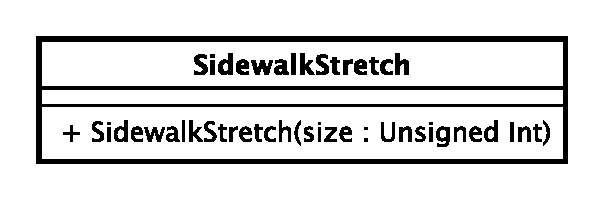
\includegraphics[scale=0.6,keepaspectratio]{images/solution/sidewalk_stretch.eps}
\caption{\pReactiveComponentStretch::SidewalkStretch}
\label{fig:sd-app-sidewalk_stretch}
\end{figure}
\FloatBarrier
\begin{itemize}
  \item \textbf{\descr} \\
    It represents a sidewalk stretch entity. It is a protected object. Only pedestrians
can tread this kind of stretch.
  \item \textbf{\ops}
    \begin{itemize}
      \item[+] \texttt{SidewalkStretch(size : Unsigned Int)} \\
        Creates a sidewalk stretch object with a specific size.
    \end{itemize}
\end{itemize}
